\documentclass[a4paper,12pt]{jarticle}
\usepackage[dvipdfmx]{graphicx}
\usepackage{amsmath,amssymb}
\usepackage{subfigure}
\usepackage{comment}
\usepackage{array}
\usepackage{setspace} % setspaceパッケージのインクルード
\usepackage{ascmac}
%\usepackage{fancybx}

\setlength{\hoffset}{0cm}
\setlength{\oddsidemargin}{-3mm}
\setlength{\evensidemargin}{-3cm}
\setlength{\marginparsep}{0cm}
\setlength{\marginparwidth}{0cm}
\setlength{\textheight}{24.7cm}
\setlength{\textwidth}{17cm}
\setlength{\topmargin}{-45pt}


\renewcommand{\baselinestretch}{1.6}
\renewcommand{\floatpagefraction}{1}
\renewcommand{\topfraction}{1}
\renewcommand{\bottomfraction}{1}
\renewcommand{\textfraction}{0}
\renewcommand{\labelenumi}{(\roman{enumi})}
%\renewcommand{\figurename}{Fig.} %図をFig.にする
\renewcommand{\baselinestretch}{1}

%図のキャプションからコロン:を消す
\makeatletter
\long\def\@makecaption#1#2{% #1=図表番号、#2=キャプション本文
\sbox\@tempboxa{#1. #2}
\ifdim \wd\@tempboxa >\hsize
#1 #2\par 
\else
\hb@xt@\hsize{\hfil\box\@tempboxa\hfil}
\fi}
\makeatother

\begin{document}
%
\title{\vspace{-30mm} \fbox{\large{計算数学特論~レポート課題2~~~機械知能工学専攻~~16344217~~津上~祐典}}}
\date{}
%
\maketitle
%
\vspace{-30mm}
%\parindent = 0pt %すべての段落で字下げをしない
%
%%%%%%%%%%%%%%%%%%%%%%%%%%%%%%%%%%%%%%%%%%%%%%%%%%%%%%%%%
\setlength{\abovedisplayskip}{0pt} % 数式上部のマージン
\setlength{\belowdisplayskip}{0pt} % 数式下部のマージン
%\setstretch{1.3} % ページ全体の行間を設定
%%%%%%%%%%%%%%%%%%%%%%%%%%%%%%%%%%%%%%%%%%%%%%%%%%%%%%%%%%

%%%%%%%%%%%%%%%%%%%%%%%%%%%%%%
\section*{課題1}
%%%%%%%%%%%%%%%%%%%%%%%%%%%%%%
\vspace{-4mm}
$p=23$の原始元は$a=7$であるので空欄を埋めると以下のようになる.
%
\begin{figure}[hbp]
 \begin{center}
  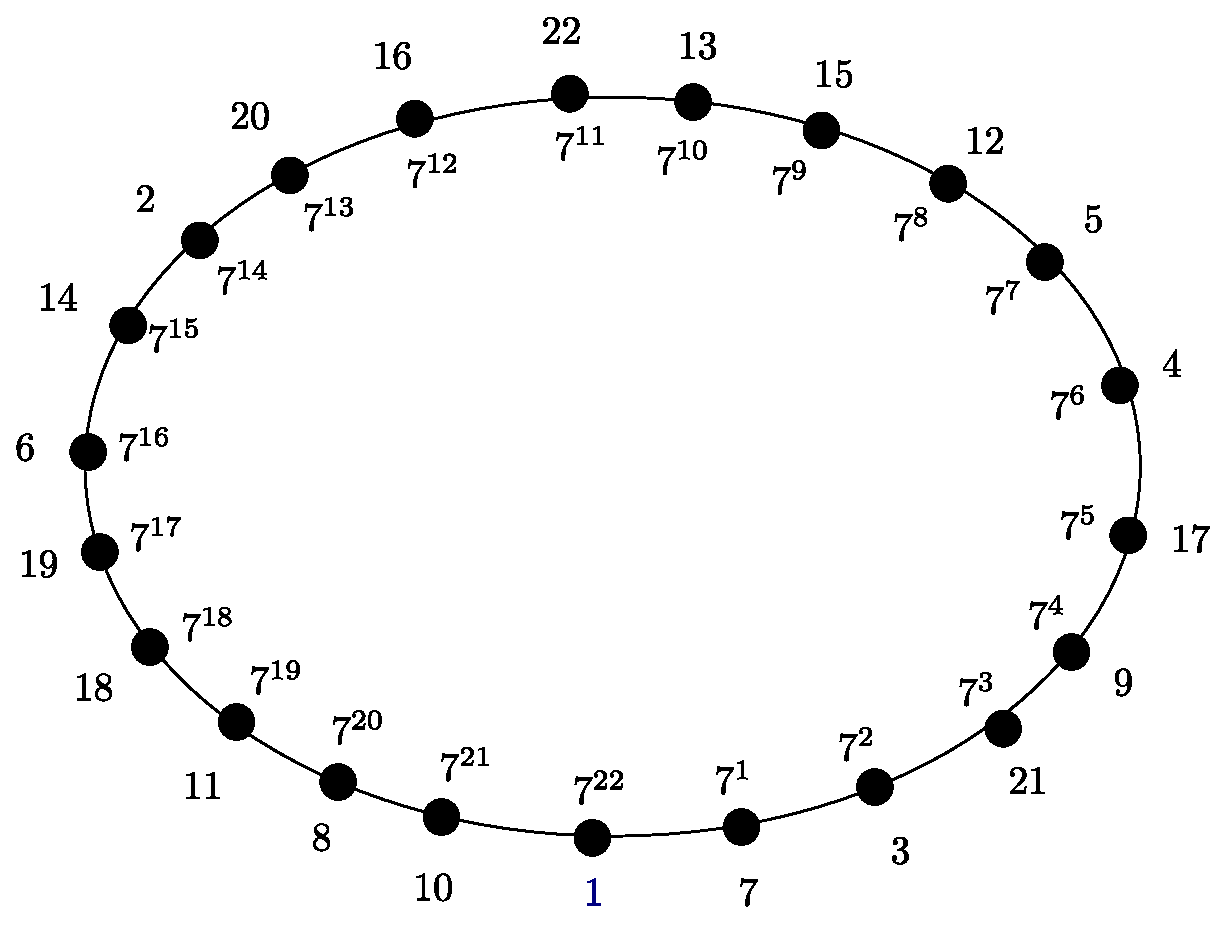
\includegraphics[width=120mm]{fig/elga.eps}
 \end{center}
 %\caption{}
 \label{fig:elga}
\end{figure}
%
\\秘密鍵を$x=20$とすると公開鍵は
%
\begin{align}
 p&=23 \\
 g&=7 \\
 y&=g^x \nonumber\\
 &=7^{20}\nonumber\\
 &=7^2\cdot7^2\cdot7^2\cdot7^2\cdot7^2\cdot7^2\cdot7^2\cdot7^2\cdot7^2\cdot7^2 \nonumber\\
  &=3\cdot3\cdot3\cdot3\cdot3\cdot3\cdot3\cdot3\cdot3\cdot3=4\cdot4\cdot4\cdot3=8
\end{align}
%
となる.次に乱数$k=9$とし$M=5$を送信する.これ暗号化すると,
%
\begin{align}
 C_1&=g^k =7^9=5\\
 C_2&=M \cdot y^k \nonumber\\
 &=5\cdot8 \cdot8^2 \cdot8^2 \cdot8^2 \cdot8^2 \nonumber\\
 &=17\cdot18 \cdot18 \cdot18 \cdot18 \nonumber\\
 &=17\cdot2 \cdot2 =22 
\end{align}
%
となる.また,復号化すると,
%
\begin{align}
 M'&=C_2\cdot \left\{ (C_1)^x \right\}^{-1} \nonumber\\
 &=22\cdot \left\{15^{20}\right\}^{-1} \nonumber\\
 &=22\cdot 15^2 \nonumber\\
 &=22\cdot18=5
\end{align}
%
となり$M$と一致する.
\vspace{-5mm}
%%%%%%%%%%%%%%%%%%%%%%%%%%%%%%
\section*{課題2}
%%%%%%%%%%%%%%%%%%%%%%%%%%%%%%
\vspace{-3mm}
%%%%%%%%%%%%%%%%%%%%%%%%%%%%%%%%%%%%%
\subsection*{(1)~$p=23$の原始元を全部求めよ.}
%%%%%%%%%%%%%%%%%%%%%%%%%%%%%%%%%%%%%
\vspace{-3mm}
$p=23$の約数は$1,2,11,22$であるので
\vspace{-6mm}
%%%%%%%%%%%%%%%%%%%%%%%%%%%%%%%%%%%%%%%
\subsection*{(2)~原始元$\alpha$,乱数$a,b$を与えて共有鍵を持てることを確認せよ.}
%%%%%%%%%%%%%%%%%%%%%%%%%%%%%%%%%%%%%%%
\vspace{-3mm}
$\alpha=7$とすると,
\end{document}
